% fov_rt_et_CONCLUSION.tex

\section{Conclusion}
The experiment scene is a mesh consisting of $12$ vertices that are indexed to create $14$ triangles, which are scaled, rotated, and translated into the scene.
This mesh is presented in figure~\ref{fig:fov}.
In order to render the scene, which rotates every given frame, the algorithm processes three reflections - thus repeating the intersection- and lighting stages of the algorithm three times per pixel.
Furthermore, the scene is lit using three pointlights; each of which may cast shadows.
During the experiment, the higher-resolution parafoveal render target is positioned in the center the screen.
As such, eye tracking in-and-of-itself had no influence on the results.

We collect elapsed times for each stage during $1000$ frames, and repeat the experiment for the foveated- and non-foveated ray tracing algorithm.
For stages computed several times (reflections with intersection- and lighting stages) we concatenate measurements.
The mean-, standard deviation-, minimum-, and maximum values of these measurements are presented in tables \ref{tab:nonfoveated} and \ref{tab:foveated}; resulting frametimes of which are presented as histograms in figures \ref{fig:histogram_non-foveated} and \ref{fig:histogram_foveated}.
The histograms present the distribution of frametimes, inside of standard deviation, in 50 bins.
The cause behind the spread of the distributions are uncertain, but might be explained by model rotation.

From measurements presented in tables \ref{tab:nonfoveated} and \ref{tab:foveated}, we may establish that foveation reduced execution time of over $90\%$ in all ray tracing stages.
This reduction is significant enough to run the ray tracer in high-definition resolutions on the target platform, and thus made it possible for us increase the previously limited application resolution.

At quick glances, the foveated rendering is not too noticable.
However, gaze position latency and aliasing issues in peripheral vision can quickly disrupt an oberver's perception of the scene, and thus pose big user experience issues.
That being said, foveation accomodating for considerably better performance may be a good-enough compromise for some applications.
As such, we conclude that performance benefits induced by foveation, demonstrated by pervious studies~\cite{guenter12} with rasterization, does extend to ray tracing.

\subsection{Future work}
Currently, the foveation algorithm causes somewhat severe overdraw, which could worsen should additional FOVs be added.
While the overdraw, using only peripheral and parafoveal render targets, causes only pixels positioned behind the high resolution render target to be redundantly evaluated, the number of redundant rays may be significantly increased with additional FOVs, especially as higher detailed FOVs would suffer overdraw.
Note, however, that the current implementation only causes overdraw of a portion of the low-resolution peripheral FOV.

Furthermore, and an issue more increasingly a problem with quality reduction of peripheral and parafoveal views, aliasing issues outside of the foveal area may cause jitter in the peripheral vision of the observer.
While advanced anti-aliasing techniques may be utilized to lessen the issue, blurring might also be a viable candidate to reduce such jitter; especially along the borders of FOVs where varying levels of quality is made particularily apperent.
An additional improvement to render foveation edges less opaque is to use a stencil algorithm to render circular FOVs.
With no corners, edge foveation differences may be less noticable.

Additionally, while consumer-level eye tracking devices are expected improve in terms of gaze positional latency and accuracy, these attributes are vital to real-time foveation to maintain the illusion of consistent quality in a scene - as the latency in garnering positional data for a gaze-contingent application, may cause an application to fall behind.
In terms of real-time rendering, this may cause foveation to lag behind; causing users to percieve lower quality renders of the scene he or she expects.

Another issue in terms of eye tracking hardware is gaze positional accuracy, which may cause high-resolution foveation to be offset erronously in relation to an observer's gaze.
In particular, this is an issue for especially small FOVs - such as a foveal render target ($2$\degree\ of the viewer's vision).
However, these hardware issues are expected to improve in the near-future; hopefully as eye tracking devices become more common in consumer-markets.

\begin{figure}[h]
  \centering
  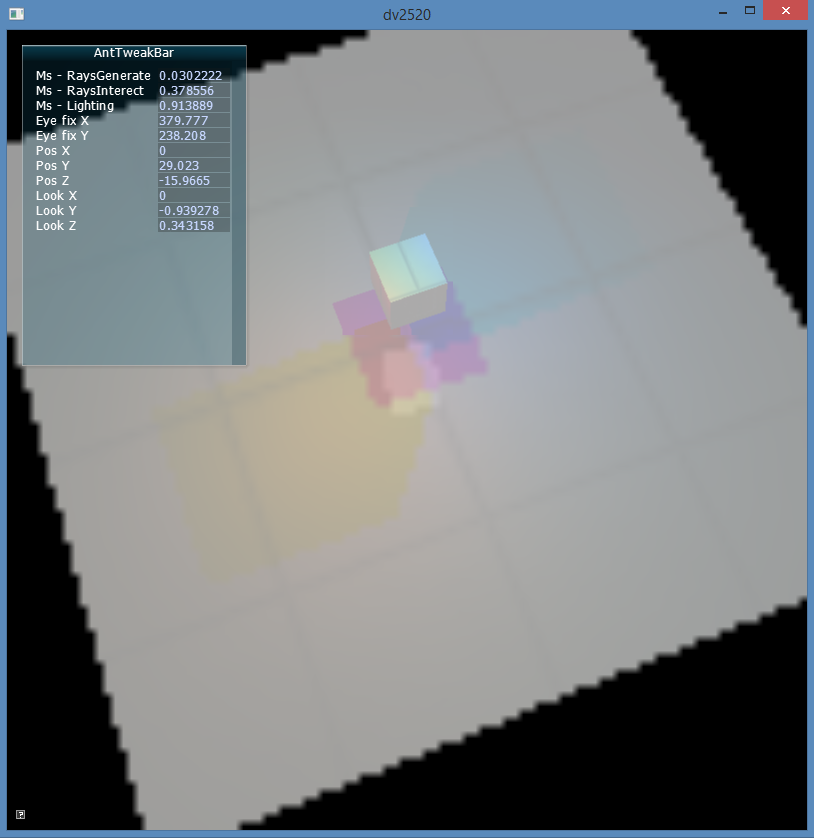
\includegraphics[width=0.75\linewidth]{img/fov_rt_et.png}
  \caption{Foveated scene. Gaze is positioned on the cube.}
  \label{fig:fov}
\end{figure}

\noindent
The author would like thank David Grelsson for contributing with the mesh used throughout the experiment.
